These checks were specified after the main study and use frozen selected
EM models (seeds 9101--9103). No learned weights or original results were
changed. Seven SNR cells and two stress cells each contain 32 fresh
worlds: 288 distinct worlds. Eight input-mismatch conditions reuse the
same 32 SNR 5~dB worlds, giving 544 condition-cases, not 544 independent
worlds. Classical and learned methods share the channel, pilots and noise.
All tests use $N=32,K=3,P=30$; the main RSR is 12~dB. The extra cells
have RSR 0~dB or two paths, at SNR 5~dB.

The small sample, post-review design and fixed checkpoints make these
exploratory checks. The intervals resample whole cases with common weights
across methods and learned seeds, separately within each cell. They are
unadjusted, conditional intervals, not a new confirmatory success test.
The original 400-case cells and their intervals remain unchanged.

\subsection{Same Candidates, Different Rank-Selection Loss}
HS-GS fits ranks 1--16 on the first 21 pilots using 25 EM updates and four
Cadzow sweeps. Exactly the same candidate channels are scored on the last
nine pilots using either squared magnitude residuals or Rician negative
log-likelihood. Each selected rank is refitted with 100 updates and all
30 pilots. This changes only the selection score, not the fit budget or
observation count. A replay against the original residual-ranked solver
agreed exactly on a fresh case; an independent likelihood check agrees
with SciPy's Rician density up to observation-only constants.

Across the seven SNR cells, Rician scoring improves HS-GS by 0.182~dB, with interval $[0.104,0.267]$~dB. 
The frozen learned estimator retains a gain of 1.282~dB, with interval $[1.092,1.485]$~dB. This score difference explains part, but not all, of the gap in this small check.

\begin{table}[!t]
\caption{Exploratory seven-SNR averages, 32 fresh cases per cell}
\centering\small
\begin{tabular}{@{}lr@{}}\toprule
Method & NMSE (dB)\\\midrule

EM100, no final filter & -10.162\\

EM100 + final hard rank six & -11.811\\

EM100 + final cubic filter & -11.648\\

EM100 + final OptShrink rank seven & -13.691\\

HS-GS, residual rank score & -12.778\\

HS-GS, Rician rank score & -12.961\\

Frozen learned model, stage-five prefix & -13.353\\

Frozen learned model, all ten stages & -14.243\\

\bottomrule\end{tabular}
\end{table}

\subsection{A Stronger Final-Filter Control}
A separate bank of 72 development worlds (eight per SNR/stress cell) selects
one global setting for each final-filter method. Selection uses only the
withheld Rician likelihood after EM100 on 21 pilots. Hard truncation and
OptShrink search ranks 1--15; cubic filtering searches relative thresholds
$\{0.01,0.03,0.1,0.3,1,3\}$. Every method also has a no-correction option.
Candidate counts differ and the grids are small; this is not an exhaustive
equal-search-budget comparison. The selected settings are rank six,
relative threshold 0.3 and OptShrink rank seven, respectively. The
settings are frozen before reading test observations, then used after
EM100 with all 30 pilots. None use true channels for tuning.

OptShrink uses the empirical spectral-tail transform in the original
algorithm~\cite{nadakuditi2014}, including rectangular zero directions and
reduced tail dimensions. A rank equal to full capacity has no tail and
is excluded; no correction is a separate candidate. At a tied boundary
within a relative squared gap of $10^{-13}$, the affected weight is set
to its zero-weight limit. Primitive checks cover zero tail, scaling,
transpose symmetry, direct rectangular trace evaluation, zero input and
the tie rule. These are numerical safeguards, not a new optimality result.

In the matched one-pass test, OptShrink beats the cubic filter by
2.042~dB on the seven-SNR average. Cubic shrinkage is therefore not
generally the best structural operation. The complete frozen learned
estimator has a 0.552~dB average gain over EM100 plus OptShrink, with
conditional interval $[0.432,0.673]$~dB. It loses 1.040~dB at SNR 20~dB
and 2.408~dB at RSR 0~dB, but gains 1.830~dB on two-path cases against
this globally selected rank-seven control. That last result does not
remove the two-path loss against per-case rank-selected HS-GS.

These comparisons have different update budgets, training/development
budgets and filtering schedules. They do not identify the best possible
OptShrink-based estimator or reproduce iterative LRHD. No controlled
runtime comparison was added; the original 64-fold timing ratio applies
only to the original HS-GS implementation.

\subsection{Reference and Noise Inputs}
The physical observations stay fixed. For amplitude errors the estimator
receives $B_{\rm in}=aB_{\rm true}$ with $a=0.9$ or $1.1$; these are
amplitude, not power, multipliers. Constant phase errors use
$B_{\rm in}=e^{j\delta}B_{\rm true}$ with $\delta=\pm10^\circ$.
The ramp uses $B_{{\rm in},np}=B_{{\rm true},np}
e^{j\delta p/(P-1)}$, $p=0,\ldots,P-1$: the assumed phase error grows
from zero to $\pm10^\circ$. Noise errors supply
$v_{\rm in}=v_{\rm true}10^{\Delta/10}$, $\Delta=\pm6$~dB.
These are input-mismatch stress tests, not measured hardware drift.
They test errors relative to a fixed true reference, not a dynamically
changing atomic receiver or a joint calibration algorithm.

\begin{table}[!t]
\caption{Input mismatch at SNR 5~dB: lower NMSE is better}
\centering\small\setlength{\tabcolsep}{5pt}
\begin{tabular}{@{}lrrr@{}}\toprule
Assumed input error & Learned & HS-Rician & Learned loss\\
 & (dB) & (dB) & vs. matched (dB)\\\midrule

None & -14.043 & -12.496 & 0.000\\

$B$ amplitude $-10\%$ & -11.613 & -9.799 & 2.430\\

$B$ amplitude $+10\%$ & -12.252 & -11.328 & 1.791\\

$B$ phase $-10^\circ$ & -11.685 & -10.730 & 2.358\\

$B$ phase $+10^\circ$ & -11.572 & -10.564 & 2.471\\

Phase ramp $0\to-10^\circ$ & -13.267 & -12.029 & 0.776\\

Phase ramp $0\to+10^\circ$ & -13.204 & -11.774 & 0.839\\

Noise variance $-6$ dB & -13.806 & -12.567 & 0.238\\

Noise variance $+6$ dB & -10.995 & -12.404 & 3.048\\

\bottomrule\end{tabular}
\end{table}

Supplying noise variance 6~dB too high worsens the learned estimate by
3.048~dB relative to matched inputs, and makes it 1.409~dB worse than
Rician-ranked HS-GS on these paired cases. This is a new observed failure,
not evidence of general variance robustness. Amplitude errors also cause
clear losses. Constant reference-phase errors rotate every estimated
channel by the same phase; replay verifies the equivariance and unchanged
phase-aligned errors. Alignment uses truth only as a diagnostic and is
not an available inference correction. Absolute-frame errors in the table
remain the reported errors.

\subsection{Depth and Controller Trajectories}
The stage-five output is taken from the unchanged ten-stage forward pass,
with its original stage feature $(t+1)/10$. It is not a five-stage model
retrained with $(t+1)/5$. Completing ten stages improves the seven-SNR
average by 0.890~dB, with interval $[0.815,0.964]$~dB; it does not help
every cell. This prefix experiment does not determine an optimal depth
or answer whether a trained twenty-stage model is better.

\begin{figure*}[!t]
\centering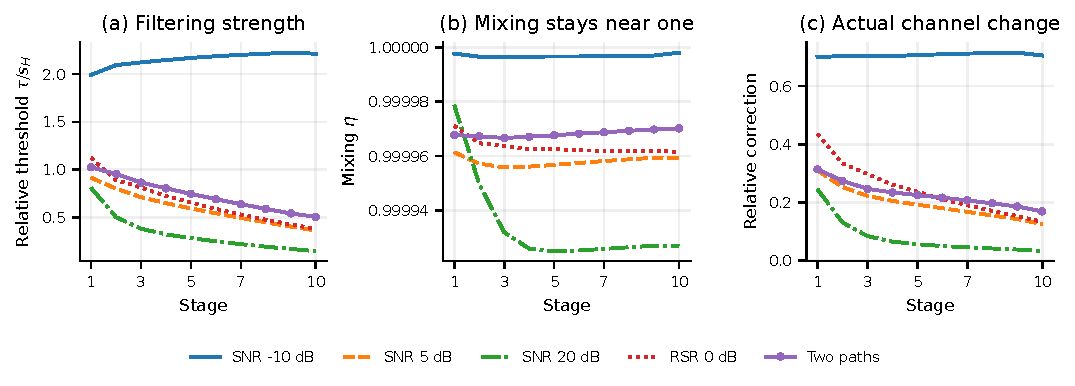
\includegraphics[width=\textwidth]{review_controller.pdf}
\caption{New frozen-model trajectories, averaged over 32 cases, three model
seeds and users. Main SNR curves use RSR 12~dB; weak-reference and two-path
curves use SNR 5~dB. All other settings are unchanged. Mixing stays near
one, while threshold and actual correction vary. Curves describe outputs;
they do not establish causal feature importance or a failure detector.}
\end{figure*}
At the ordinary SNR 5~dB condition the mean relative threshold falls from
about 0.915 at stage one to 0.362 at stage ten. Mean mixing is about
0.99996. Thus the useful adaptation is primarily in threshold strength,
not abstention. Large relative corrections in a failure condition do not
prove which feature or prior caused the failure.

